\documentclass[11pt]{article}
\usepackage{homework}
\let\div\relax
\usepackage{mathabx}

\classname{444}
\homeworknum{6}


\DeclareMathAlphabet{\mathsfit}{T1}{\sfdefault}{\mddefault}{\sldefault}



\begin{document}

% Environments

\newcommand{\state}[2]{\begin{statement}{#1} #2 \end{statement}}
\newcommand{\prob}[2]{\begin{problem}{#1} #2 \end{problem}}
\newcommand{\subprob}[1]{\begin{subproblem} #1 \end{subproblem}}
\newcommand{\sol}[1]{\begin{solution} #1 \end{solution}}
\newcommand{\fig}[2]{\begin{figure} \centering #2  \label{#1} \end{figure}}

\newcommand{\makebib}{
	\vfill
	\color{black}
	\nocite{*}
	\bibliography{references}{}
	\bibliographystyle{lucas_unsrt}
}
	

% Implication

\newcommand{\qwhere}{\quad \text{where} \quad}
\newcommand{\qimplies}{\quad \implies \quad}
\newcommand{\impliesq}{\implies \quad}



% Brackets

\newcommand{\paren}[1]{\left( #1 \right)}
\newcommand{\brac}[1]{\left[ #1 \right]}
\newcommand{\curly}[1]{\left\{ #1 \right\}}


% Greek

\newcommand{\alp}{\alpha}
\newcommand{\bet}{\beta}
\newcommand{\gam}{\gamma}
\newcommand{\del}{\delta}
\newcommand{\eps}{\epsilon}
\newcommand{\zet}{\zeta}
\newcommand{\tht}{\theta}
\newcommand{\kap}{\kappa}
\newcommand{\lam}{\lambda}
\newcommand{\sig}{\sigma}
\newcommand{\ups}{\upsilon}
\newcommand{\omg}{\omega}

\newcommand{\Gam}{\Gamma}
\newcommand{\Del}{\Delta}
\newcommand{\Tht}{\Theta}
\newcommand{\Lam}{\Lambda}
\newcommand{\Sig}{\Sigma}
\newcommand{\Omg}{\Omega}


% Text

\newcommand{\where}{\text{where }}

% Problem 1

\newcommand{\Hint}{H_\text{int}}
\newcommand{\ddcx}{\dd[3]{x}}
\newcommand{\psib}{\bar{\psi}}

\newcommand{\mh}{m_h}
\newcommand{\mmu}{m_\mu}
\newcommand{\me}{m_e}
\newcommand{\ma}{m_a}

\newcommand{\aexpt}{a_\text{expt.}}
\newcommand{\aQED}{a_\text{QED}}
\renewcommand{\GeV}{\giga\electronvolt}

\newcommand{\gamt}{\gam^5}



\state{The Bertotti-Robsinson solution of the Einstein field equation~(MCP 26.2)}{
	Bruno Bertotti and Ivor Rovinson independently solved the Einstein field equation to obtain the following metric for a universe endowed with a uniform magnetic field:
	\eqn{given1}{
		\dds^2 = Q^2 (-\ddt^2 + \sin^2 t \ddz^2 + \ddtht^2 + \sin^2\tht \ddphi^2).
	}
	Here
	\al{
		Q &= \const, &
		0 &\leq t \leq \pi, &
		-\infty &< z < +\infty, &
		0 &\leq \tht \leq \pi, &
		0 &\leq \phi \leq 2\pi.
	}
%	If one computes the Einstein tensor from the metric coefficients of the line element Eq.~\refeq{given1} and equates it to $8\pi$ times a stress-energy tensor, one finds a stress-energy tensor that is precisely the same as for an electromagnetic field lifted, unchanged, into general relativity.  The electromagnetic field is one that, as measured in the local Lorentz frame of an observer with fixed $\{ z, \tht, \phi \}$ (a ``static'' observer), has vanishing electric field and has a magnetic field directed along $\pdv*{z}$ with magnitude independent of where the observer is located in spacetime.  In this sense, the spacetime metric Eq.~\refeq{given1} is that of a homogeneous magnetic universe.  
Discuss the geometry of this universe and the nature of the coordinates $\{ t, z, \tht, \phi \}$.
}

\prob{
	Which coordinate increases in a timelike direction and which coordinates in spacelike directions?
}

\sol{
	The coordinate $t$ increases in a timelike direction because $\ddt^2$ appears in the metric with a minus sign.  The coordinates $z$, $\tht$, and $\phi$ all increase in a spacelike direction because $\ddz^2$, $\ddtht^2$, and $\ddphi^2$ appear in the metric with plus signs.
}



\prob{
	Is this universe spherically symmetric?
}

\sol{
	Yes.  We can think of $\{ \tht, \phi \}$ as a coordinate system on the 2-surface of constant $t$ and $z$.  The metric for this 2-surface is
	\eq{
		\spw \dds^2 = Q^2 (\ddtht^2 + \sin^2\tht \dd\phi^2),
	}
	which is the line element of a 2-dimensional sphere in spherical coordinates.  This means the spacetime in Eq.~\refeq{given1} is spherically symmetric~\cite[p.~1244]{MCP}.
}



\prob{
	Is this universe cylindrically symmetric?
}

\sol{
	No.  In order for the universe to be cylindrically symmetric, we would need a constant-$r$ 2-surface parametrized by some coordinates $\{ \phh, \zh \}$ with the line element
	\eq{
		\spw \dds^2 = r^2 \dd{\phh}^2 + \dd{\zh}^2.
	}
	This does not appear in Eq.~\refeq{given1}.
}



\prob{
	Is this universe asymptotically flat?
}

\sol{
	No.  In order for the spacetime to be asymptotically flat, we would need to find some limit in which Eq.~\refeq{given1} took the form
	\eq{
		\dds^2 = -\ddt^2 + \ddx^2 + \ddy^2 + \ddz^2.
	}
	No such limit exists.
}



\prob{
	How does the geometry of this universe change as $t$ ranges from $0$ to $\pi$?  [Hint: show that the curves $\{ z, \tht, \phi = \const,\ t = \tau / Q \}$ are timelike geodesics---the world lines of the static observers referred to above.  Then argue from symmetry, or use the result of Ex.~25.4a.]
}

\sol{
	A timelike geodesic has a tangent vector $\vuu$ which can be normalized such that $\vuu = \dv*{\tau}$~\cite[p.~1202]{MCP}.  The geodesic equation is $\nabvuu \vuu = 0$ by MCP~(25.11d).
}



\prob{
	Give as complete a characterization as you can of the coordinates $\{ t, z, \tht, \phi \}$.
}






\clearpage
\newcommand{\Fab}{F^{\alp \bet}}
\newcommand{\Ua}{U^\alp}
\newcommand{\Usa}{U_\alp}
\newcommand{\Ub}{U^\bet}
\newcommand{\Xa}{X^\alp}
\newcommand{\Xsa}{X_\alp}
\newcommand{\Xb}{X^\bet}
\newcommand{\xap}{x^\alp_p}
\newcommand{\xaq}{x^\alp_q}

\begin{statement}{(Jackson 11.17)}
	The electric and magnetic fields \refeq{fields} of a charge in uniform motion can be obtained from Coulomb's law in the charge's rest frame and the fact that the field strength $\Fab$ is an antisymmetric tensor of rank 2 without considering \emph{explicitly} the Lorentz transformation.  The idea is the following.  For a charge in uniform motion the only relevant variables are the charge's 4-velocity $\Ua$ and the relative coordinate $\Xa = \xap - \xaq$, where $\xap$ and $\xaq$ are the 4-vector coordinates of the observation point and the charge, respectively.  The only antisymmetric tensor that can be formed is $(\Xa \Ub - \Xb \Ua)$.  Thus the electromagnetic field $\Fab$ must be this tensor multiplied by some scalar function of the possible scalar products, $\Xsa \Xa$, $\Xsa \Ua$, $\Usa \Ua$.
\end{statement}

\newcommand{\vbb}{\vb{b}}
\newcommand{\vv}{\vb{v}}
\newcommand{\Eq}{E_1}
\newcommand{\Ew}{E_2}
\newcommand{\Ee}{E_3}
\newcommand{\Bq}{B_1}
\newcommand{\Bw}{B_2}
\newcommand{\Be}{B_3}

\newcommand{\xsq}{x^1}


\begin{figure} \centering
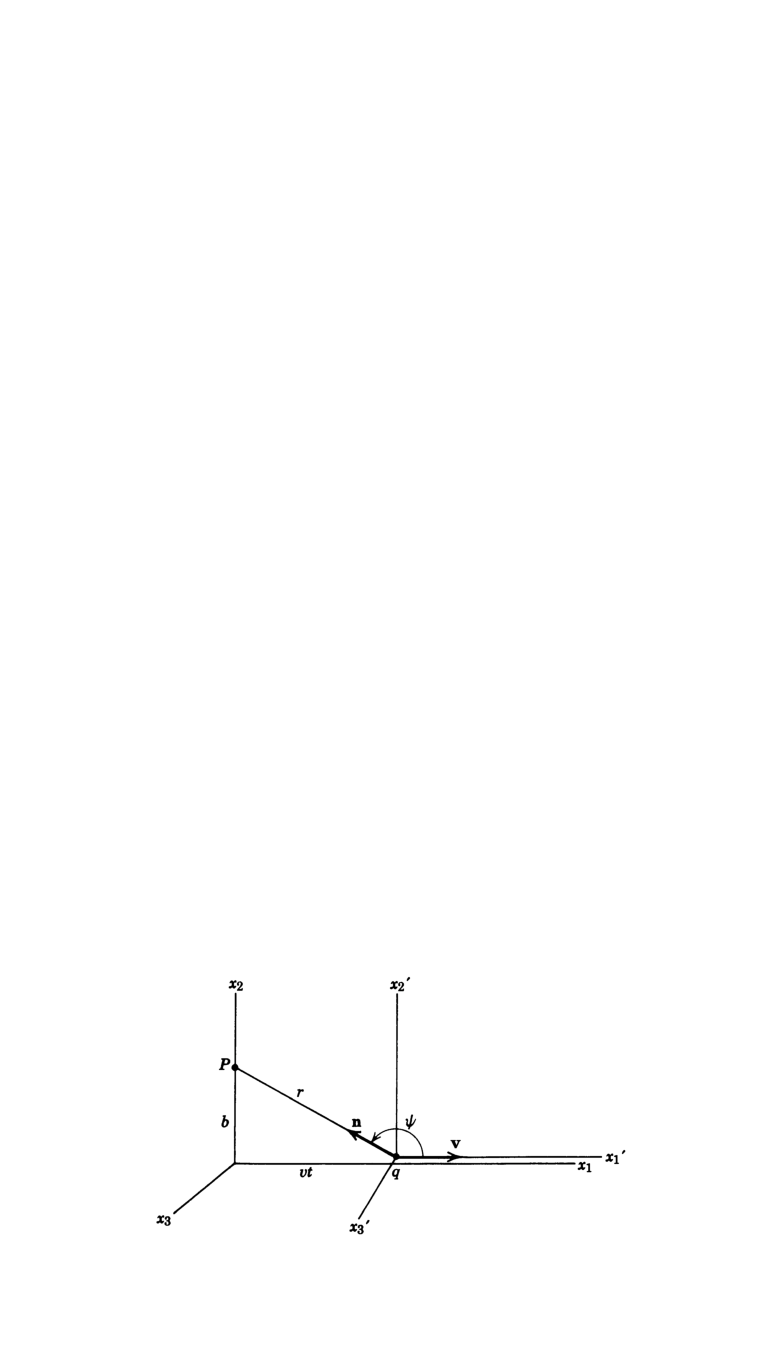
\includegraphics{11-8}
\caption{(Jackson Fig.~11.8) Particle of charge $q$ moving at constant velocity $\vv$ passes an observation point $P$ at impact parameter $b$.}
\label{11.8}
\end{figure}

\begin{problem} \label{2.a}
	For the geometry of Fig.~\ref{11.8} the coordinates of $P$ and $q$ at a common time in $K$ can be written $\xap = (ct, \vbb)$, $\xaq = (ct, \vv t)$, with $\vbb \vdot \vv = 0$.  By considering the general form of $\Fab$ in the rest frame of the charge, show that
	\beqn \label{show2.a}
		\Fab = \frac{q}{c} \frac{\Xa \Ub - \Xb \Ua}{[(\Usa \Xa / c)^2 - \Xsa \Xa]^{3/2}}.
	\eeqn
	Verify that this yields the expressions
	\begin{align} \label{fields}
		\Eq &= \Eq' = -\frac{q \gam v t}{(b^2 + \gam^2 v^2 t^2)^{3/2}}, &
		\Ew &= \gam \Ew' = \frac{\gam q b}{(b^2 + \gam^2 v^2 t^2)^{3/2}}, &
		\Be &= \gam \bet \Ew' = \bet \Ew,
	\end{align}
	with all other components vanishing, in the inertial frame $K$.
\end{problem}


\newcommand{\Fmat}{\mqty[	0 & -\Eq & -\Ew & -\Ee \\
						\Eq & 0 & -\Be & \Bw \\
						\Ew & \Be & 0 & -\Bq \\
						\Ee & -\Bw & \Bq & 0 ]}
\newcommand{\Fpab}{{F'}^{\alp\bet}}
\newcommand{\rp}{{r'}}
\newcommand{\tLam}{\tilde{\Lam}}
\newcommand{\Lammat}{\mqty[\gam & \gam \beta & 0 & 0 \\	
						\gam \beta & \gam & 0 & 0 \\
						0 & 0 & 1 & 0 \\
						0 & 0 & 0 & 1 ]}

\begin{solution}
	From Jackson~(11.137),
	\beqn \label{F}
		\Fab = \Fmat,
	\eeqn
	and from the equation immediately preceding Jackson~(11.151),
	\begin{align*}
		\Eq' &= -\frac{q v t'}{\rp^3}, &
		\Ew' &= \frac{q b}{\rp^3}, &
		\Ee' &= 0, &
		\Bq' &= 0, &
		\Bw' &= 0, &
		\Be' &= 0,
	\end{align*}
	in the rest frame of the charge for the geometry in Fig.~\ref{1}.  Here, $r' = \sqrt{b^2 + v^2 {t'}^2}$.  Then, in $K'$,
	\beqn \label{thing2.1b}
		\Fpab = \frac{q}{(b^2 + v^2 {t'}^2)^{3/2}}
			\mqty[0 & v t' & -b & 0 \\
				-v t' & 0 & 0 & 0 \\
				b & 0 & 0 & 0 \\
				0 & 0 & 0 & 0 ].
	\eeqn
	Now we will boost into the frame $K$.  From Jackson~(11.147), $F' = \Lam F \tLam$, although we need $F = \Lam F' \tLam$, where we boost in the direction opposite the particle's motion.  According to Jackson~(11.113), the Lorentz boost in the $-x'$ direction is
	\beqn \label{Lam2}
		\Lam = \Lammat.
	\eeqn
	Then
	\begin{align*}
		\Fab &= \frac{q}{(b^2 + v^2 {t'}^2)^{3/2}} \Lammat
			\mqty[ 0 & v t' & -b & 0 \\
				-v t' & 0 & 0 & 0 \\
				b & 0 & 0 & 0 \\
				0 & 0 & 0 & 0 ]
			\Lammat \\
		&= \frac{q}{(b^2 + v^2 {t'}^2)^{3/2}}
			\mqty[ -\gam \bet v t' & \gam v t' & -\gam b & 0 \\
				-\gam v t' & \gam \bet v t' & -\gam \bet b & 0 \\
				b & 0 & 0 & 0 \\
				0 & 0 & 0 & 0 ]
			\Lammat
		= \frac{q}{(b^2 + v^2 {t'}^2)^{3/2}}
			\mqty[ 0 & v t' & -\gam b & 0 \\
				-v t' & 0 & -\gam \bet b & 0 \\
				\gam b & \gam \bet b & 0 & 0 \\
				0 & 0 & 0 & 1 ].
	\end{align*}
	From \refeq{lorentz}, $t' = \gam t$ since $x = 0$.  Finally,
	\beqn \label{thing2.1}
		\Fab = \frac{\gam q}{(b^2 + \gam^2 v^2 t^2)^{3/2}} 
			\mqty[0 & v t & -b & 0 \\
				-v t & 0 & -v b / c & 0 \\
				b & v b / c & 0 & 0 \\
				0 & 0 & 0 & 0 ].
	\eeqn
	
	Now we will begin from \refeq{show2.a} and find $\Fab$ directly in $K$.  In accordance with Fig.~\ref{11.8},
	\begin{align*}
		\Xa &= (0, \vbb - \vv t) = (0, -v t, b, 0), &
		\Ua &= \gam (c, \vv) = \gam (c, v, 0, 0),
	\end{align*}
	and so
	\beq
		\Xa \Ub - \Xb \Ua = \gam
			\mqty[ 0 & 0 & 0 & 0 \\
				-c v t & -v^2 t & 0 & 0 \\
				c b & v b & 0 & 0 \\
				0 & 0 & 0 & 0 ]
		- \gam
			\mqty[ 0 & -c v t & c b & 0 \\
				0 & -v^2 t & v b & 0 \\
				0 & 0 & 0 & 0 \\
				0 & 0 & 0 & 0 ]
		= \gam
			\mqty[0 & c v t & - c b & 0 \\
				-c v t & 0 & -v b & 0 \\
				c b & v b & 0 & 0 \\
				0 & 0 & 0 & 0 ].
	\eeq
	Additionally,
	\begin{align*}
		\Usa \Xa &= \gam \mqty[ c & -v & 0 & 0 ] \mqty[ 0 \\ -v t \\ b \\ 0 ]
		= \gam v^2 t, &
		\Xsa \Xa &= \mqty[ 0 & vt & -b & 0 ] \mqty[ 0 \\ -v t \\ b \\ 0 ]
		= -v^2 t^2 - b^2.
	\end{align*}
	Then, applying \refeq{show2.a},
	\beq
		\Fab = \frac{\gam q}{(\gam^2 v^4 t^2 / c^2 + v^2 t^2 + b^2)^{3/2}}
			\mqty[0 & v t & -b & 0 \\
				-v t & 0 & -v b / c & 0 \\
				b & v b / c & 0 & 0 \\
				0 & 0 & 0 & 0 ].
	\eeq
	Note that
	\beq
		v^2 t^2 + \frac{\gam^2 v^4 t^2}{c^2} = v^2 t^2 \left( 1 + \gam^2 \frac{v^2}{c^2} \right)
		= v^2 t^2 \left( 1 + \frac{\bet^2}{1 - \bet^2} \right)
		= v^2 t^2 \frac{1 - \bet^2 + \bet^2}{1 - \bet^2}
		= \gam^2 v^2 t^2,
	\eeq
	so we have again arrived at \refeq{thing2.1}.  Thus, we have proven \refeq{show2.a}.
	
	In addition, comparing \refeq{thing2.1} with \refeq{F}, we see that
	\begin{align*}
		\Eq &= -\frac{q \gam v t}{(b^2 + \gam^2 v^2 t^2)^{3/2}}, &
		\Ew &= \frac{\gam q b}{(b^2 + \gam^2 v^2 t^2)^{3/2}}, &
		\Be &= \frac{\gam \bet q b}{(b^2 + \gam^2 v^2 t^2)^{3/2}} = \bet \Ew.
	\end{align*}
	Comparing \refeq{thing2.1b} with \refeq{F} as well, and making the substitution $t' = \gam t$, yields
	\begin{align*}
		\Eq' &= -\frac{q \gam v t}{(b^2 + \gam^2 v^2 t^2)^{3/2}}, &
		\Ew' &= \frac{q b}{(b^2 + \gam^2 v^2 t^2)^{3/2}},
	\end{align*}
	so we have also verified \refeq{fields}. \qed
\end{solution}


\newcommand{\xpap}{{x'}^\alp_p}
\newcommand{\xpaq}{{x'}^\alp_q}
\newcommand{\Ya}{Y^\alp}
\newcommand{\Ysa}{Y_\alp}
\newcommand{\Yb}{Y^\bet}
\newcommand{\Ypa}{{Y'}^\alp}

\begin{problem}
	Repeat the calculation, using as the starting point the common-time coordinates in the rest frame, ${\xpap = (ct', \vbb - \vv t')}$ and $\xpaq = (ct', 0)$.  Show that
	\beqn \label{show2.b}
		\Fab = \frac{q}{c} \frac{\Ya \Ub - \Yb \Ua}{(- \Ysa \Ya)^{3/2}},
	\eeqn
	where $\Ypa = \xpap - \xpaq$.  Verify that the fields are the same as in \ref{2.a}.  Note that to obtain the results of \refeq{fields} it is necessary to use the time $t$ of the observation point $P$ in $K$ as the time parameter.
\end{problem}

\newcommand{\Ypsa}{{Y'}_\alp}
\newcommand{\Ypb}{{Y'}^\bet}
\newcommand{\Upa}{{U'}^\alp}
\newcommand{\Upb}{{U'}^\bet}
\newcommand{\vo}{\mathbf{0}}
\newcommand{\tp}{{t'}}

\begin{solution}
	Firstly, note that
	\begin{align*}
		\Ypa &= (0, \vbb - \vv t') = (0, -v t', b, 0), &
		\Upa &= (c, \vo) = (c, 0, 0, 0),
	\end{align*}
	Then
	\beq
		\Ypa \Upb - \Ypb \Upa = c
			\mqty[ 0 & 0 & 0 & 0 \\
				-v t' & 0 & 0 & 0 \\
				b & 0 & 0 & 0 \\
				0 & 0 & 0 & 0 ]
		- c
			\mqty[ 0 & -v t' & b & 0 \\
				0 & 0 & 0 & 0 \\
				0 & 0 & 0 & 0 \\
				0 & 0 & 0 & 0 ]
		= c
			\mqty[ 0 & v t' & -b & 0 \\
				-v t' & 0 & 0 & 0 \\
				b & 0 & 0 & 0 \\
				0 & 0 & 0 & 0 ],
	\eeq
	and
	\beq
		\Ypsa \Ypa = \mqty[ 0 & v t' & -b & 0 ] \mqty[ 0 \\ -v t' \\ b \\ 0 ] = -v^2 \tp^2 - b^2,
	\eeq
	so, from \refeq{show2.b}, in $K'$ we have
	\beq
		\Fpab = \frac{q}{(b^2 + v^2 \tp^2)^{3/2}}
			\mqty[ 0 & v t' & -b & 0 \\
				-v t' & 0 & 0 & 0 \\
				b & 0 & 0 & 0 \\
				0 & 0 & 0 & 0 ],
	\eeq
	which is identical to \refeq{thing2.1b}.  We know that boosting into $K$ yields \refeq{thing2.1}.
	
	Now we will find $\Fab$ directly in $K$ by boosting $\Ypa$ and $\Upa$.  From Jackson~(11.84), $x' = \Lam x$ (where $x$ represents $x^\alp$), and we once again use $\Lam$ given by \refeq{Lam2} to perform $x = \Lam x'$.  We obtain
	\begin{align*}
		Y &= \Lam Y'
		= \Lammat \mqty[ 0 \\ -v t' \\ b \\ 0]
		= \mqty[ -\gam \bet v t' \\ -\gam v t' \\ b \\ 0 ], &
		U &= \Lam U'
		= \Lammat \mqty[ c \\ 0 \\ 0 \\ 0 ]
		= \gam c \mqty[ 1 \\ \bet \\ 0 \\ 0 ].
	\end{align*}
	Then
	\beq
		\Ya \Ub - \Yb \Ua = \gam c
			\mqty[ -\gam \bet v t' & -\gam \bet^2 v t' & 0 & 0 \\
				-\gam v t' & -\gam \bet v t' & 0 & 0 \\
				b & \bet b & 0 & 0 \\
				0 & 0 & 0 & 0 ]
			- \gam c
			\mqty[ -\gam \bet v t' & -\gam v t' & b & 0 \\
				-\gam \bet^2 v t' & -\gam \bet v t' & \bet b & 0 \\
				0 & 0 & 0 & 0 \\
				0 & 0 & 0 & 0 ]
		= c
			\mqty[ 0 & v t' & -\gam b & 0 \\
				-v t' & 0 & -\gam \bet b & 0 \\
				\gam b & \gam \bet b & 0 & 0 \\
				0 & 0 & 0 & 0 ],
	\eeq
	and
	\beq
		\Ysa \Ya = \mqty[ -\gam \bet v t' & \gam v t' & -b & 0] \mqty[ -\gam \bet v t' \\ -\gam v t' \\ b \\ 0 ]
		= \gam^2 \bet^2 v^2 \tp^2 - \gam^2 v^2 \tp^2 - b^2
		= -v^2 \tp^2 - b^2.
	\eeq
	Making these substitutions into \refeq{show2.b}, and using $t' = \gam t$,
	\beq
		\Fab = \frac{q}{(b^2 + v^2 \tp^2)^{3/2}}
			\mqty[ 0 & v t' & -\gam b & 0 \\
				-v t' & 0 & -\gam v b / c & 0 \\
				\gam b & \gam v b / c & 0 & 0 \\
				0 & 0 & 0 & 0 ]
		= \frac{\gam q}{(b^2 + \gam^2 v^2 t^2)^{3/2}}
			\mqty[ 0 & v t & -b & 0 \\
				-v t & 0 & -v b / c & 0 \\
				b & v b / c & 0 & 0 \\
				0 & 0 & 0 & 0 ],
	\eeq
	which is identical to \refeq{thing2.1}, and therefore gives the fields from \refeq{fields} as in \ref{2.a}.  Thus, we have proven \refeq{show2.b}. \qed
\end{solution}


\newcommand{\Za}{Z^\alp}
\newcommand{\Zsa}{Z_\alp}
\newcommand{\Zb}{Z^\bet}
\newcommand{\vbet}{\boldsymbol{\beta}}

\begin{problem}
	Finally, consider the coordinate $\xap = (ct, \vbb)$ and the ``retarded-time'' coordinate $\xaq = [ct - R, \vbet(ct - R)]$ where $R$ is the distance between $P$ and $q$ at the retarded time.  Define the difference as $\Za = [R, \vbb - \vbet(ct - R)]$.  Show that in terms of $\Za$ and $\Ua$ the field is
	\beqn \label{show2.c}
		\Fab = \frac{q}{c} \frac{\Za \Ub - \Zb \Ua}{(\Usa \Za / c)^3}.
	\eeqn
\end{problem}
\vfix

\begin{solution}
	Referring to Fig~\ref{11.8},
	\begin{align*}
		\Za &= (R, \vbb - \vv t + \vv R / c) = [R, -v (t - R / c), b, 0], &
		\Ua &= \gam (c, \vv) = \gam (c, v, 0, 0).
	\end{align*}
	Then
	\begin{align*}
		\Za\Ub - \Zb \Ua &= \gam
			\mqty[c R & R v & 0 & 0 \\
				-v (c t - R) & -v^2 (t - R / c) & 0 & 0 \\
				c b & b v & 0 & 0 \\
				0 & 0 & 0 & 0 ]
			- \gam
			\mqty[ c R & -v (c t - R) & c b & 0 \\
				R v & -v^2 (t - R / c) & b v & 0 \\
				0 & 0 & 0 & 0 \\
				0 & 0 & 0 & 0 ] \\
		&= \gam c
			\mqty[0 & v t & -b & 0 \\
				-v t & 0 & -v b / c & 0 \\
				b & v b / c & 0 & 0 \\
				0 & 0 & 0 & 0 ],
	\end{align*}
	and
	\beq
		\Usa \Za = \gam \mqty[ c & -v & 0 & 0 ] \mqty[ R \\ -v (t - R / c) \\ b \\ 0 ]
		= \gam cR + \gam v^2(t - R/c),
	\eeq
	so
	\beq
		\frac{\Usa \Za}{c} = \gam R + \gam \bet^2 c t - \gam \bet^2 R
		= (1 - \bet^2) \gam R + \gam \bet^2 c t
		= \frac{R}{\gam} + \gam \bet^2 c t.
	\eeq
	
	Note that $\xap$ and $\xaq$, as they are defined here, have lightlike separation since $R / c$ is, by definition, the time it takes light to travel from $\xaq$ to $\xap$.  Then
	\beq
		0 = \Zsa \Za
		= \mqty[ R & v (t - R / c) & -b & 0 ] \mqty[ R \\ -v (t - R / c) \\ b \\ 0 ]
		= R^2 - v^2 (t - R / c)^2 - b^2,
	\eeq
	which implies
	\beq
		R^2 = b^2 + v^2 (t - R / c)^2.
	\eeq
	This is corroborated by the geometry of Fig.~\ref{11.8}, since $t - R / c$ is the retarded time.  Then, referring to the denominator of \refeq{thing2.1}, we find
	\begin{align*}
		b^2 + \gam^2 v^2 t^2 &= R^2 - v^2 (t - R / c)^2 + \gam^2 v^2 t^2
		= R^2 - \bet^2  (c^2 t^2 - 2 R c t + R^2) + \gam^2 \bet^2 c^2 t^2 \\
		&= (1 - \bet^2) R^2 + 2 R \bet^2 c t + (\gam^2 - 1) \bet^2 c^2 t^2
		= \frac{R^2}{\gam^2} + 2 R \bet^2 c t + \gam^2 \bet^4 c^2 t^2
		= \left( \frac{R}{\gam} + \gam \bet^2 c t \right)^2 \\
		&= \left( \frac{\Usa \Za}{c} \right)^2.
	\end{align*}
	In summary, we have found
	\beq
		\Fab = \frac{\gam q}{(b^2 + \gam^2 v^2 t^2)^{3/2}}
			\mqty[0 & v t & -b & 0 \\
				-v t & 0 & -v b / c & 0 \\
				b & v b / c & 0 & 0 \\
				0 & 0 & 0 & 0 ],
	\eeq
	which is identical to \refeq{thing2.1}.  Thus, we have proven \refeq{show2.c}. \qed
\end{solution}







\state{Mass-radius relation for neutron stars~(MCP 26.7)}{
%	The equation of state of a neutron star is very hard to calculate at the supra-nuclear densities required, because the calculation is a complex, many-body problem and the particle interactions are poorly understood an poorly measured.  Observations of neutron stars' masses and radii can therefore provide valuable constraints on fundamental nuclear physics.  As we discuss briefly in the following chapter, various candidate equations of state can already be excluded on these observational grounds.
	
%	A necessary step for comparing observation with theory is to compute the stellar structure for candidate equations of state.  
	We can illustrate the approach using a simple functional form, which, around nuclear density ($\rhonuc \simeq \SI{2.3e17}{\kg\per\cubic\meter}$), is a fair approximation to some of the models:
	\eq{
		P = \num{3e32} \paren{ \frac{\rho}{\rhonuc} }^3 \:\si{\newton\per\square\meter}.
	}
	For this equation of state, use the equations of stellar structure~(26.38a) and (26.38c) to find the masses and radii of stars with a range of central pressures, and hence deduce a mass-radius relation, $M(R)$.  You should discover that, as the central pressure is increased, the mass passes through a maximum, while the radius continues to decrease.
}

\sol{
	MCP~(26.38a) and (26.38c) are, respectively,
	\al{
		\dv{m}{r} &= 4 \pi r^2 \rho, &
		\dv{P}{r} &= -\frac{(\rho + P) (m + 4\pi r^3 P)}{r (r - 2m)}.
	}
	\hl{what are we even supposed to do here?}
}






\clearpage
\state{}{
	An astronaut on a rocket ship has just crossed the event horizon of a Schwarzschild black hole.  Show that, no matter how the rocket engines are fired, they will reach $r = 0$ in a proper time $\tau \leq \pi M$.
}




\clearpage
\state{Fermat's principle for a photon's path in static spacetime~(MCP~27.4)}{
	Show that the Euler-Lagrange equation for the action principle,
	\eqn{27.8}{
		\Del t = \intoq \sqrt{ \gamjk \dv{\xj}{\eta} \dv{\xk}{\eta} } \ddeta,
		\qquad \text{where }
		\gamjk = \frac{\sgjk}{-\sgoo},
	}
	is equivalent to the geodesic equation for a photon in the static spacetime metric $\sgoo(\xk)$, $\sgij(\xk)$.  Specifically, do the following.
}

\prob{
	The action~Eq.~\refeq{27.8} is the same as that for a geodesic in a 3-dimensional space with the metric $\gamjk$ and with $t$ playing the role of proper distance traveled~[Eq.~(25.19) converted to a positive-definite, 3-dimensional metric].  Therefore, the Euler-Lagrange equation for Eq.~\refeq{27.8} is the geodesic equation in that (fictitious) space [Eq.~(25.14) with $t$ the affine parameter].  Using Eq.~(24.38c) for the connection coefficients, show that the geodesic equation can be written in the form
	\eqn{show5a}{
		\gamjk \dv[2]{\xk}{t} + \frac{1}{2} (\gamjkl + \gamjlk - \gamklj) \dv{\xk}{t} \dv{\xl}{t} = 0.
	}
}

\sol{
	MCP~(25.14) is
	\eqn{25.14}{
		\dv[2]{\xalp}{\zet} + \Gam^\alp{}_{\mu \nu} \dv{\xmu}{\zet} \dv{\xnu}{\zet} = 0
	}
	with $\zet$ the affine parameter.  With $t$ as the affine parameter, this can be written
	\eq{
		0 = \dv[2]{x_j}{t} + \Gam_{j k l} \dv{\xk}{t} \dv{\xl}{t}
		= \sgjk \dv[2]{\xk}{t} + \Gam_{j k l} \dv{\xk}{t} \dv{\xl}{t},
	}
	where we have also lowered the first index.  Using the definition $\gamjk = \sgjk / {-\sgoo}$, we can write
	\eqn{thing5a}{
		\gamjk \dv[2]{\xk}{t} + \frac{1}{-\sgoo} \Gam_{j k l} \dv{\xk}{t} \dv{\xl}{t}.
	}
	MCP~(24.28c) is
	\eq{
		\Gam_{\alp \bet \gam} = \frac{1}{2} (\sg_{\alp \bet, \gam} + \sg_{\alp \gam, \bet} - \sg_{\bet \gam, \alp} + c_{\alp \bet \gam} + c_{\alp \bet \gam} - c_{\bet \gam \alp}).
	}
	Assuming a coordinate basis, the commutation coefficients $c_{\alp \bet \gam}$ vanish~\cite[p.~1171]{MCP}.  Then, again using the definition of $\gamjk$, we have
	\eq{
		\frac{1}{-\sgoo} \Gam_{j k l} = \frac{1}{2} (\gam_{j k, l} + \gam_{j l, k} - \gam_{k l, j}).
	}
	Making this substitution in Eq.~\refeq{thing5a}, we have
	\eq{
		\ans{ \gamjk \dv[2]{\xk}{t} + \frac{1}{2} (\gamjkl + \gamjlk - \gamklj) \dv{\xk}{t} \dv{\xl}{t} = 0 }
	}
	as desired. \qed
}



\prob{
	Take the geodesic equation~Eq.~\refeq{25.14} for the light ray in the real spacetime, with spacetime affine parameter $\zet$, and change parameters to coordinate time $t$.  Thereby obtain
	\aln{ \label{show5b}
		\sgjk \dv[2]{\xk}{t} + \Gamjkl \dv{\xk}{t} \dv{\xl}{t} - \Gamjoo \frac{\sgkl}{\sgoo} \dv{\xk}{t} \dv{\xl}{t} + \frac{\dv*[2]{t}{\zet}}{(\dv*{t}{\zet})^2} \sgjk \dv{\xk}{t} &= 0, &
		\frac{\dv*[2]{t}{\zet}}{(\dv*{t}{\zet})^2} + 2 \Gamoko \frac{\dv*{\xk}{t}}{\sgoo} &= 0.
	}
}



\prob{
	Insert the second of Eqs.~\refeq{show5b} into the first, and write the connection coefficients in terms of derivatives of the spacetime metric.  With a little algebra, bring your result into the form Eq.~\refeq{show5a} of the Fermat-principle Euler-Lagrange equation.
}






\state{}{
	Consider a collapsing spherical shell of dust with radius $R(\tau)$ where $\tau$ is the proper time of the dust.  Exterior to the shell the metric is Schwarzschild with some mass parameter $M$, while interior the geometry is that of flat empty space.
}

\prob{
	Show that the rest mass of the shell, $\mu = 4 \pi R^2(\tau) \sig$ is constant, where $\sig$ is the surface mass density.
}



\prob{
	Derive a differential equation of motion for $R(\tau)$:
	\eq{
		M = \mu \sqrt{ 1 + \paren{ \dv{R}{\tau} }^2 } - \frac{\mu^2}{2 R}.
	}
}



\prob{
	Solve the equation (implicitly) in the special case where the dust begins collapse at rest from infinite radius.
}


\makebib

\end{document}
